\section{System Architecture}
\label{sec:architecture}

\subsection{Overall Architecture}

LectureMind follows a three-tier architecture consisting of a React frontend, Django backend, and storage layer. Figure~\ref{fig:architecture} shows the component relationships.

\begin{figure}[H]
    \centering
    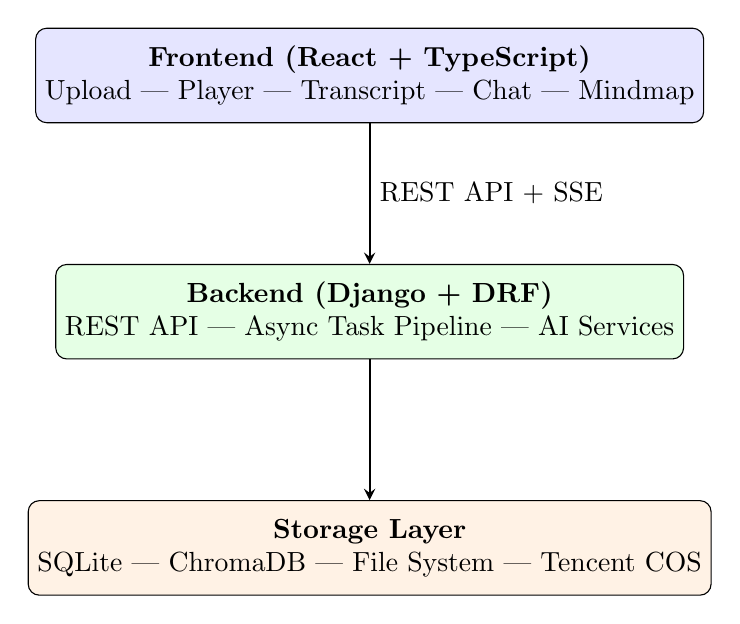
\begin{tikzpicture}[
        node distance=2cm,
        box/.style={rectangle, draw, rounded corners, minimum width=4cm, minimum height=1.2cm, align=center},
        arrow/.style={->, >=stealth, thick}
    ]
        % Frontend
        \node[box, fill=blue!10, minimum width=8cm] (frontend) {
            \textbf{Frontend (React + TypeScript)} \\
            Upload | Player | Transcript | Chat | Mindmap
        };
        
        % Backend
        \node[box, fill=green!10, below of=frontend, yshift=-1cm] (backend) {
            \textbf{Backend (Django + DRF)} \\
            REST API | Async Task Pipeline | AI Services
        };
        
        % Storage
        \node[box, fill=orange!10, below of=backend, yshift=-1cm] (storage) {
            \textbf{Storage Layer} \\
            SQLite | ChromaDB | File System | Tencent COS
        };
        
        % Arrows
        \draw[arrow] (frontend) -- node[right] {REST API + SSE} (backend);
        \draw[arrow] (backend) -- (storage);
    \end{tikzpicture}
    \caption{Three-Tier System Architecture}
    \label{fig:architecture}
\end{figure}

\subsection{Async Task Pipeline}

The core processing logic is implemented as a DAG-based async task pipeline. Each task is represented as a database record with dependency tracking, enabling parallel execution where possible and proper sequencing where required.

\subsubsection{Task Data Model}

Tasks are stored in the \texttt{AsyncTaskItem} model:

\begin{lstlisting}[language=Python, caption={AsyncTaskItem Database Model}]
class AsyncTaskItem(models.Model):
    id = UUIDField(primary_key=True)
    video = ForeignKey(Video)
    task_type = CharField(max_length=100)
    status = CharField(
        choices=['pending', 'running', 'success', 'error']
    )
    previous = ForeignKey('self', null=True)
    input_data = JSONField(default=dict)
    result_data = JSONField(default=dict)
    error_message = TextField(blank=True)
    error_type = CharField(max_length=100, blank=True)
    created_at = DateTimeField(auto_now_add=True)
    started_at = DateTimeField(null=True)
    completed_at = DateTimeField(null=True)
\end{lstlisting}

The \texttt{previous} field establishes the dependency chain. When a task completes successfully, any task depending on it becomes eligible for execution.

\subsubsection{Task Processor}

The task processor is implemented as a Django management command that continuously polls for pending tasks:

\begin{lstlisting}[language=Python, caption={Async Task Processor Loop}, label={alg:task-processor}]
while running:
    acquire database lock
    select pending tasks where previous task is complete
    if task found:
        mark task as running
        release lock
        execute task function
        if success:
            mark task as success
            merge result into dependent task's input
        else:
            mark task as error
            cascade error to all dependent tasks
    else:
        release lock
        sleep for 5 seconds
\end{lstlisting}

The processor uses \texttt{SELECT FOR UPDATE SKIP LOCKED} to support multiple concurrent workers safely. This row-level locking ensures that no two workers process the same task simultaneously.

\subsubsection{Task DAG}

Figure~\ref{fig:task-dag} illustrates the complete task dependency graph.

\begin{figure}[H]
    \centering
    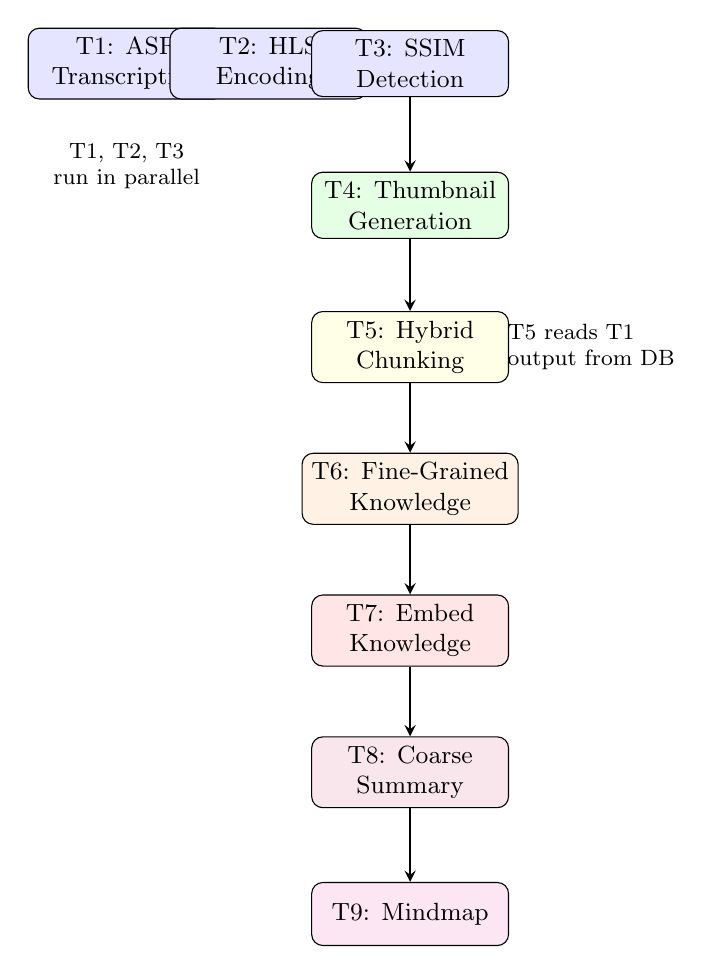
\begin{tikzpicture}[
        node distance=1.8cm,
        task/.style={rectangle, draw, rounded corners, minimum width=2.5cm, minimum height=0.8cm, align=center, font=\small},
        arrow/.style={->, >=stealth, thick}
    ]
        % Level 1 (parallel)
        \node[task, fill=blue!10] (t1) {T1: ASR\\Transcription};
        \node[task, fill=blue!10, right of=t1] (t2) {T2: HLS\\Encoding};
        \node[task, fill=blue!10, right of=t2] (t3) {T3: SSIM\\Detection};
        
        % Level 2
        \node[task, fill=green!10, below of=t3] (t4) {T4: Thumbnail\\Generation};
        
        % Level 3
        \node[task, fill=yellow!10, below of=t4] (t5) {T5: Hybrid\\Chunking};
        
        % Level 4
        \node[task, fill=orange!10, below of=t5] (t6) {T6: Fine-Grained\\Knowledge};
        
        % Level 5
        \node[task, fill=red!10, below of=t6] (t7) {T7: Embed\\Knowledge};
        
        % Level 6
        \node[task, fill=purple!10, below of=t7] (t8) {T8: Coarse\\Summary};
        
        % Level 7
        \node[task, fill=magenta!10, below of=t8] (t9) {T9: Mindmap};
        
        % Arrows
        \draw[arrow] (t3) -- (t4);
        \draw[arrow] (t4) -- (t5);
        \draw[arrow] (t5) -- (t6);
        \draw[arrow] (t6) -- (t7);
        \draw[arrow] (t7) -- (t8);
        \draw[arrow] (t8) -- (t9);
        
        % Note about T1 dependency
        \node[below of=t1, yshift=0.5cm, font=\footnotesize, align=center] {T1, T2, T3\\run in parallel};
        \node[right of=t5, xshift=0.5cm, font=\footnotesize, align=left] {T5 reads T1\\output from DB};
    \end{tikzpicture}
    \caption{Task Dependency Graph (DAG)}
    \label{fig:task-dag}
\end{figure}

\subsection{Data Models}

The system uses several core data models to represent processed content:

\begin{itemize}
    \item \textbf{Video:} Metadata about uploaded videos (title, duration, file path, processing status)
    \item \textbf{VideoTranscript:} ASR output with language detection and overall statistics
    \item \textbf{TranscriptSentence:} Individual sentences with timestamps, emotions, and language codes
    \item \textbf{Thumbnail:} Screenshots extracted at slide transition points
    \item \textbf{VideoSection:} Intelligent segments produced by hybrid chunking
    \item \textbf{KnowledgePoint:} Fine-grained knowledge extracted per section
    \item \textbf{KnowledgeSummary:} Coarse-grained lecture-level summary
    \item \textbf{KnowledgeMindmap:} Hierarchical concept map data
    \item \textbf{ChatSession/ChatMessage:} Conversation history for RAG interactions
\end{itemize}
